\documentclass[a4paper]{article}
\usepackage{graphicx}
\usepackage[a4paper, margin=2cm]{geometry}
\setlength{\parindent}{0pt}

\title{Lab 3 - Report}
\author{rayane guerou}

\begin{document}

\maketitle

\section{CPU greyscale}

\begin{figure}[h!]
\centering
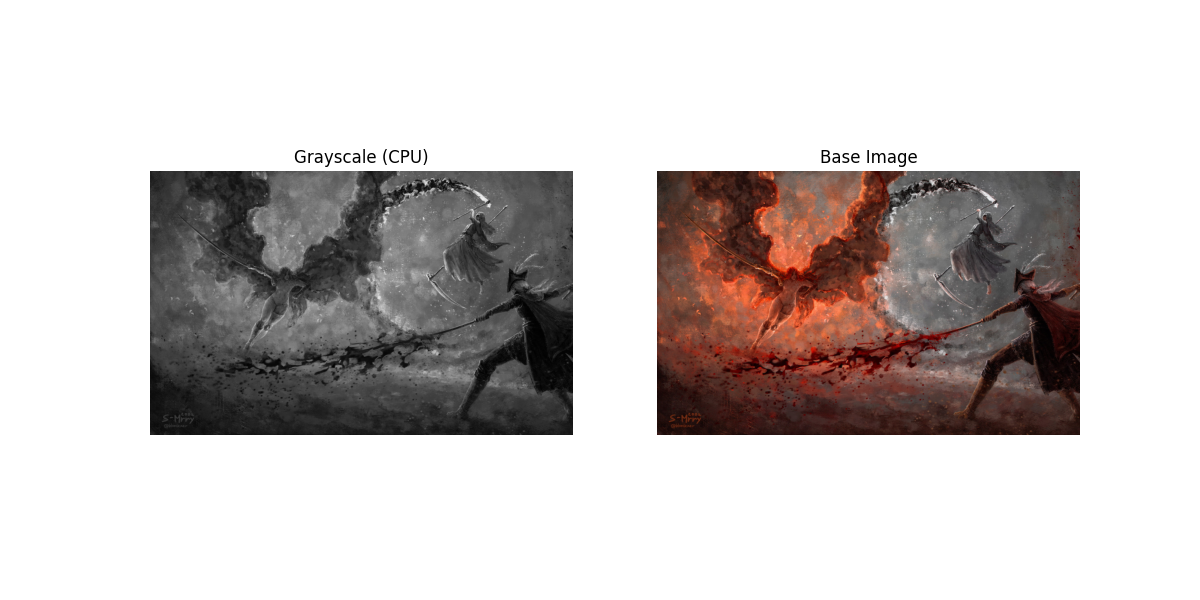
\includegraphics[scale=0.4]{../src/grayscale_cpu.png}
\caption{CPU greyscale comparaison}
\end{figure}
\vspace{1cm}

\section{GPU greyscale}
We first import an image, then for convert it to grayscale with CUDA gpu and then we resize the image then with the grayscale kernel 

\begin{figure}[h!]
\centering
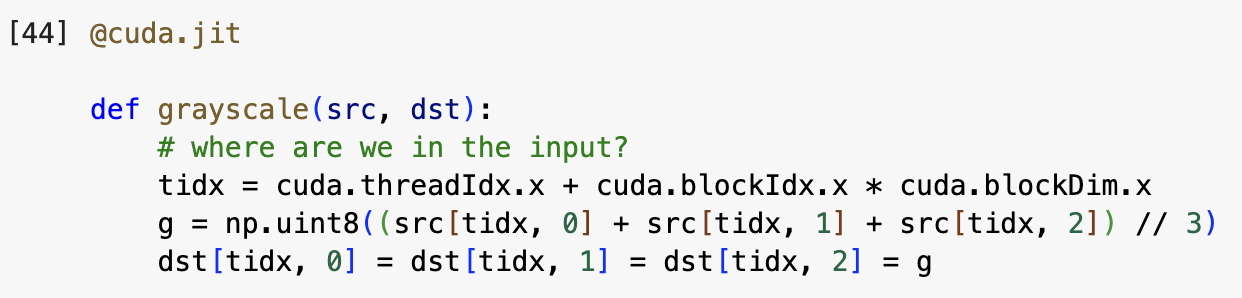
\includegraphics[scale=0.5]{../src/grayscale.png}
\caption{CPU greyscale code}
\end{figure}

We can now convert it to grayscale using the GPU and display it, so we see it's working and very faster than the CPU one
\vspace{5cm}
\section{GPU block size comparaison}

We now try different block size to compare the execution time with GPU and block size

\begin{figure}[h]
    \centering
    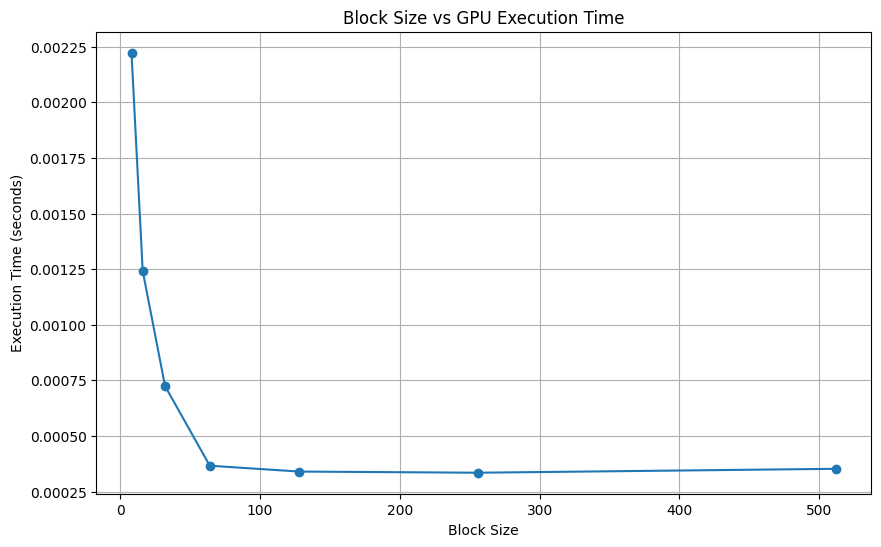
\includegraphics[scale=0.5]{../src/block_size.png}
    \caption{CPU greyscale code}
    \end{figure}



We can see that the execution time converges rapidly to 0.00035s, 
so we can deduce that it's not necessarily useful to set too large a block size

\end{document}
